\documentclass[11pt, a4paper]{article}
\usepackage{graphicx}
\usepackage{amsmath}
\usepackage{listings}


\title{Assignment 6: 1D Simulation of a tubelight}
\author{G Ch V Sairam , EE19B081}
\date{10-04-2021}

\begin{document}		
		
\maketitle
\section*{Introduction}
Python is very good at simulating models. We use a 1-D model of a tubelight.A uniform electric field is present, that accelerates electrons. Electrons are emitted by the cathode with zero energy, and accelerate in this field. When they get beyond a threshold energy $E_0$ , they can drive atoms to excited states. The relaxation of these atoms results in light emission. Electrons reaching the anode are absorbed and lost. Each “time step”, an average of N electrons are introduced at the cathode.

\section*{Simulation}
We create a simulation universe. The tube is divided into n sections. In each time instant, M electrons are injected. We run the simulation for nk turns. The electrons excite only after the atoms reach a velocity of u0. Beyond this velocity, there is a probability p in each turn that a collision will occur and an atom excited. The excited electron’s velocity reduces to zero if it collides.

\lstinputlisting[language=Python,firstline=37,lastline=65]{EE19B081_assign6.py}

\section*{Plots}
We plot the histograms of Electron Density and Light Emission Intensity and the plot of electron phasespace.

\begin{figure}[!tbh]
\centering
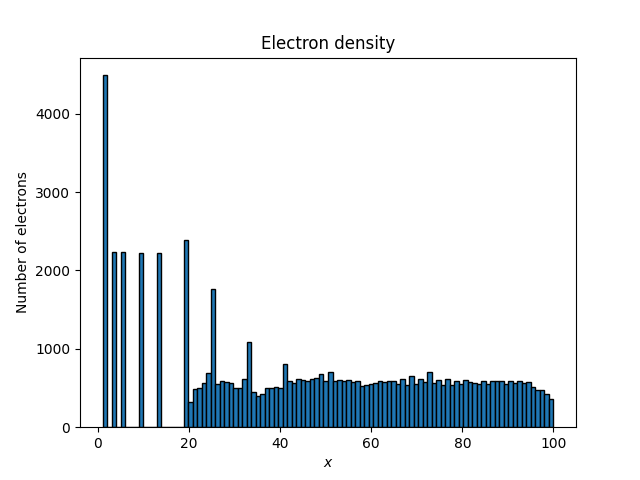
\includegraphics[scale=0.75]{assn6_plot0.png} 
\caption{Electron density histogram}
\label{fig0}
\end{figure}

\begin{figure}[!tbh]
\centering
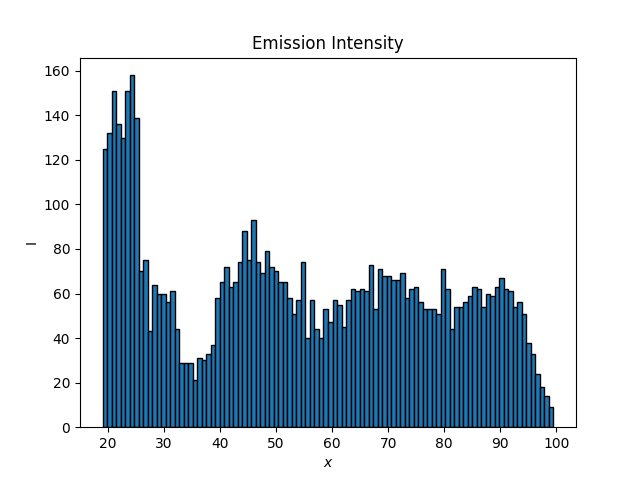
\includegraphics[scale=0.75]{assn6_plot1.png} 
\caption{Emission intensity histogram}
\label{fig1}
\end{figure}

\begin{figure}[!tbh]
\centering
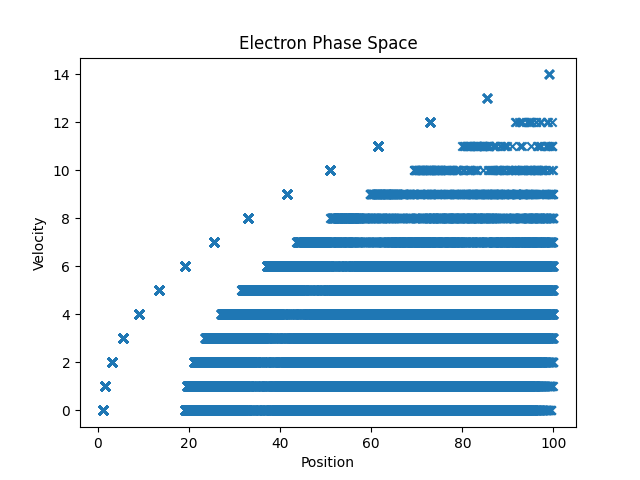
\includegraphics[scale=0.7]{assn6_plot2.png} 
\caption{Electron phase space}
\label{fig2}
\end{figure}

\section*{Intensity table}
The emission count for each value of x is tabulated below:
\begin{verbatim*}
Intensity data:
xpos	count
19.41	125
20.21	132
21.02	151
21.82	136
22.63	130
23.43	151
24.24	158
25.04	139
25.85	70
26.65	75
27.46	43
28.26	64
29.07	60
29.87	60
30.68	56
31.48	61
32.29	44
33.09	29
33.9	29
34.7	29
35.51	21
36.31	31
37.12	30
37.92	33
38.73	37
39.53	58
40.34	65
41.14	72
41.95	63
42.75	65
43.56	74
44.36	88
45.17	75
45.97	93
46.78	74
47.58	69
48.39	79
49.19	72
50.0	70
50.8	65
51.61	65
52.41	58
53.22	51
54.02	57
54.83	74
55.63	40
56.44	57
57.24	44
58.05	40
58.85	53
59.66	47
60.46	57
61.27	55
62.07	45
62.88	57
63.68	62
64.49	61
65.29	62
66.1	61
66.9	73
67.71	53
68.51	71
69.32	68
70.12	68
70.93	66
71.73	66
72.54	69
73.34	58
74.15	62
74.95	63
75.76	56
76.56	53
77.37	53
78.17	53
78.98	51
79.78	71
80.59	62
81.39	44
82.2	54
83.0	54
83.81	56
84.61	59
85.42	63
86.22	62
87.03	54
87.83	60
88.64	59
89.44	63
90.25	67
91.05	62
91.86	61
92.66	54
93.47	56
94.27	51
95.08	38
95.88	33
96.69	24
97.49	18
98.3	14
99.1	9
\end{verbatim*}

\section*{Conclusion}
We use python to simulate models for various requirements. Here,we used it to simualte electron motion in a tubelight, and hence find out the illumination
at different points.

We can make the following conclusions from varying the parameters and observe the various plots that arise:
\begin{itemize}
\item For low threshold speed, photon emission starts occuring from a much lower value of x.
\item A gas which has a lower threshold velocity and a higher ionization probability is better suited for use in a tubelight since it provides more uniform and a higher amount of photon emission intensity.

\end{itemize}

\end{document}